% (C) Marc Lijour, 2017 
% Licensed under a Creative Commons License BY-SA
% https://creativecommons.org/licenses/by-sa/2.5/ca/
% Presentation for the Pathway to Prosperity (P2P) Conference, November 16, 2017
% see http://p2pcanada.ca/library/pathways-to-prosperity-2017-national-conference/
% authored by Marc Lijour, November 2017
% 
% Variables
% TODO set the variables
% ---------------------- USER-DEFINED --------------------------------
\newcommand{\ICTCtitle}{Outiller les jeunes agents de changement}
\newcommand{\ICTClongtitle}{Guider les jeunes agents du changement num\'erique}
%\newcommand{\ICTClongtitle}{Guider les jeunes agents du changement numérique}
\newcommand{\ICTCsubtitle}{Atelier sur le mentorat (Conf\'erence Pathways to Prosperity 2017)}
\newcommand{\ICTCauthor}{Marc~Lijour}
\newcommand{\ICTCdate}{16 novembre 2017}
\newcommand{\ICTCsubject}{INPE}
% --------------------------------------------------------------------
% Template
%% (C) Marc Lijour, 2017
% This document is licensed under a Creative Commons License BY-SA (feel free to use the code, but all rights are reserved for logos and art)
% https://creativecommons.org/licenses/by-sa/2.5/ca/
% ICTC presentation template in LaTeX
% This template comes with a first page on a picture background
% Possible improvement in future iterations
% - Test and fix as needed to work on xetex (to use Ubuntu fonts)
% === USAGE===
% Create a file for your LaTeX content (slides, etc), in which you must do the following:
% TODO 1 - set variables defined below
% TODO 2 - include this code by calling: \input{<the name of this document>}
% TODO 3 - Start the document as usual and you're in business; just use \begin{document} and don't forget to conclude with \end{document}
% TODO 4 - Use the custom method \ICTCcoverpage instead of \titlepage to create your cover page
% Voilà!
%
\documentclass[utf8]{beamer}
\usepackage{etoolbox}
%\usepackage[american,french]{babel}
%\usepackage[T1]{fontenc}
%\usepackage[utf8]{inputenc}
% Variables
% ---------------------- USER-DEFINED --------------------------------
\ifdef{\ICTCtitle}{}{\newcommand{\ICTCtitle}{\color{red}Title TBD}}
\ifdef{\ICTClongtitle}{}{\newcommand{\ICTClongtitle}{\color{red}Long title TBD}}
\ifdef{\ICTCsubtitle}{}{\newcommand{\ICTCsubtitle}{\color{red}Subtitle TBD}}
\ifdef{\ICTCauthor}{}{\newcommand{\ICTCauthor}{\color{red}Author TBD}}
\ifdef{\ICTCdate}{}{\newcommand{\ICTCdate}{\color{red}Date TBD}}
\ifdef{\ICTCsubject}{}{\newcommand{\ICTCsubject}{\color{red}Subject TBD}}
% --------------------------------------------------------------------
\usetheme{Boadilla}
% Set color close to ICTC paletter
\definecolor{beamer@blendedblue}{RGB}{220,0,66}
% Cover Page
\title[\ICTCtitle] {\ICTClongtitle}
\subtitle{\ICTCsubtitle}
\author{\ICTCauthor}
\date{\ICTCdate}
\subject{\ICTCsubject}
\usepackage{tikz}
% Try Xetex to use system fonts (pdflatex makes it hard to import a font)
%\usepackage{fontspec}
%\setsansfont{Ubuntu}
%\setmonofont{Ubuntu Mono}

% -- create a custom (command) title page -which has the benefit of not affecting the settings for the rest of the presentation
\newcommand{\ICTCcoverpage}{\frame[plain]{
	\tikz[remember picture,overlay] {
        	\node(bkgd) at ([xshift=0cm,yshift=0cm]current page.center) 
			{
\includegraphics[width=\paperwidth, height=\paperheight]{../../ICTC-LaTeX_Templates/images/ictc-canada}};
        	\node(logo) at ([xshift=0cm,yshift=1.8cm]current page.center) 
%		 	{
\includegraphics[scale=.15]{../../ICTC-LaTeX_Templates/images/ICTC-logo-TM-NN-medium_400x400-transparent-whiteletters}};
		 	{
\includegraphics[scale=.4]{../../pics/logos/ICTC_logo_TRANS_white_letters}};
        	\node(CC-BY-SA) at ([xshift=5cm,yshift=-3.5cm]current page.center) 
			{\href{https://creativecommons.org/licenses/by-sa/2.5/ca/}{
\includegraphics[scale=.4]{../../ICTC-LaTeX_Templates/images/CC-BY-SA-403x141}}};
	}
	\tikz[remember picture,overlay] {
        	\node(title) at ([xshift=0cm,yshift=0cm]current page.center) 
			{\Large\color{white}\textbf{{\ICTClongtitle}}};
        	\node(subtitle) at ([xshift=0cm,yshift=-.7cm]current page.center) 
			{\small\color{white}\emph{\ICTCsubtitle}};
        	\node(author) at ([xshift=0cm,yshift=-2cm]current page.center) 
			{\small\color{white}By~\ICTCauthor};
        	\node(date) at ([xshift=0cm,yshift=-2.5cm]current page.center) 
			{\tiny\color{white}\ICTCdate};
        	\node(footnote) at ([xshift=0cm,yshift=-4cm]current page.center) 
			{\TINY\color{white}\emph{The Information and Communications Technology Council (ICTC) is a centre of expertise on the digital economy}};
        	\node(footnote) at ([xshift=0cm,yshift=-4.2cm]current page.center) 
			{\TINY\color{white}\emph{with 25+ years of research on the ICT sector and the labour market}};
    	}
}}
%
% This sets the ICTC logo at the bottom right corner of each page
\logo{
	
\includegraphics[scale=.08]{../../ICTC-LaTeX_Templates/images/ICTC-logo-TM-NN-medium_400x400-onwhite}
}
\AtBeginSection[]
{
  \begin{frame}
    \frametitle{Table of Contents}
    \tableofcontents[currentsection]
  \end{frame}
}
%\usepackage{newunicodechar}
%\usepackage[format=plain,justification=raggedright,singlelinecheck=false]{caption}
\usepackage[format=plain,justification=justified,singlelinecheck=false]{caption}
\usepackage{dirtytalk}
\usepackage{wrapfig}
\usepackage{hyperref}
\usepackage{verbatim}
\usepackage{mathabx}
%\usepackage{MnSymbol}


% (C) Marc Lijour, 2017
% This document is licensed under a Creative Commons License BY-SA (feel free to use the code, but all rights are reserved for logos and art)
% https://creativecommons.org/licenses/by-sa/2.5/ca/
% ICTC presentation template in LaTeX
% This template comes with a first page on a picture background
% Possible improvement in future iterations
% - Test and fix as needed to work on xetex (to use Ubuntu fonts)
% === USAGE===
% Create a file for your LaTeX content (slides, etc), in which you must do the following:
% TODO 1 - set variables defined below
% TODO 2 - include this code by calling: \input{<the name of this document>}
% TODO 3 - Start the document as usual and you're in business; just use \begin{document} and don't forget to conclude with \end{document}
% TODO 4 - Use the custom method \ICTCcoverpage instead of \titlepage to create your cover page
% Voilà!
%
\documentclass[utf8]{beamer}
\usepackage{etoolbox}
%\usepackage[american,french]{babel}
%\usepackage[T1]{fontenc}
%\usepackage[utf8]{inputenc}
% Variables
% ---------------------- USER-DEFINED --------------------------------
\ifdef{\ICTCtitle}{}{\newcommand{\ICTCtitle}{\color{red}Title TBD}}
\ifdef{\ICTClongtitle}{}{\newcommand{\ICTClongtitle}{\color{red}Long title TBD}}
\ifdef{\ICTCsubtitle}{}{\newcommand{\ICTCsubtitle}{\color{red}Subtitle TBD}}
\ifdef{\ICTCauthor}{}{\newcommand{\ICTCauthor}{\color{red}Author TBD}}
\ifdef{\ICTCdate}{}{\newcommand{\ICTCdate}{\color{red}Date TBD}}
\ifdef{\ICTCsubject}{}{\newcommand{\ICTCsubject}{\color{red}Subject TBD}}
% --------------------------------------------------------------------
\usetheme{Boadilla}
% Set color close to ICTC paletter
\definecolor{beamer@blendedblue}{RGB}{220,0,66}
% Cover Page
\title[\ICTCtitle] {\ICTClongtitle}
\subtitle{\ICTCsubtitle}
\author{\ICTCauthor}
\date{\ICTCdate}
\subject{\ICTCsubject}
\usepackage{tikz}
% Try Xetex to use system fonts (pdflatex makes it hard to import a font)
%\usepackage{fontspec}
%\setsansfont{Ubuntu}
%\setmonofont{Ubuntu Mono}

% -- create a custom (command) title page -which has the benefit of not affecting the settings for the rest of the presentation
\newcommand{\ICTCcoverpage}{\frame[plain]{
	\tikz[remember picture,overlay] {
        	\node(bkgd) at ([xshift=0cm,yshift=0cm]current page.center) 
			{
\includegraphics[width=\paperwidth, height=\paperheight]{../../ICTC-LaTeX_Templates/images/ictc-canada}};
        	\node(logo) at ([xshift=0cm,yshift=1.8cm]current page.center) 
		 	{
\includegraphics[scale=.15]{../../ICTC-LaTeX_Templates/images/ICTC-logo-TM-NN-medium_400x400-transparent-whiteletters}};
        	\node(CC-BY-SA) at ([xshift=5cm,yshift=-3.5cm]current page.center) 
			{\href{https://creativecommons.org/licenses/by-sa/2.5/ca/}{
\includegraphics[scale=.4]{../../ICTC-LaTeX_Templates/images/CC-BY-SA-403x141}}};
	}
	\tikz[remember picture,overlay] {
        	\node(title) at ([xshift=0cm,yshift=0cm]current page.center) 
			{\Large\color{white}\textbf{{\ICTClongtitle}}};
        	\node(subtitle) at ([xshift=0cm,yshift=-.7cm]current page.center) 
			{\small\color{white}\emph{\ICTCsubtitle}};
        	\node(author) at ([xshift=0cm,yshift=-2cm]current page.center) 
			{\small\color{white}Présenté par~\ICTCauthor};
        	\node(date) at ([xshift=0cm,yshift=-2.5cm]current page.center) 
			{\tiny\color{white}le~\ICTCdate};
        	\node(footnote) at ([xshift=0cm,yshift=-4cm]current page.center) 
			{\TINY\color{white}\emph{Le Conseil des Technologies de l'information et des communications (CTIC) est un centre national d'expertise sans but lucratif}};
        	\node(footnote) at ([xshift=0cm,yshift=-4.2cm]current page.center) 
			{\TINY\color{white}\emph{dont la mission est d'assurer l'avantage compétitif du Canada dans le secteur numérique.}};
    	}
}}
%
% This sets the ICTC logo at the bottom right corner of each page
\logo{
	
\includegraphics[scale=.1]{../../ICTC-LaTeX_Templates/images/ICTC-logo-TM-NN-medium_400x400-onwhite}
}
\AtBeginSection[]
{
  \begin{frame}
    \frametitle{Table of Contents}
    \tableofcontents[currentsection]
  \end{frame}
}
%\usepackage{newunicodechar}
%\usepackage[format=plain,justification=raggedright,singlelinecheck=false]{caption}
\usepackage[format=plain,justification=justified,singlelinecheck=false]{caption}
\usepackage{dirtytalk}
\usepackage{wrapfig}
\usepackage{hyperref}
\usepackage{verbatim}
\usepackage{mathabx}
%\usepackage{MnSymbol}


% Extra packages
\usepackage{amssymb}
\usepackage{amsmath}
\usepackage{csquotes}
\usepackage[american,french]{babel}
\usepackage[backend=biber,style=apa]{biblatex}
\DeclareLanguageMapping{american}{american-apa}
% Use one bib file per section
%\addbibresource{references-program-overview.bib}
\addbibresource{references-p2p-mentorat.bib}
\definecolor{links}{HTML}{2A1B81}
\hypersetup{colorlinks,linkcolor=,urlcolor=links}
% special purpose
\newcommand*\rfrac[2]{{}^{#1}\!/_{#2}}
% Start of the document
\begin{document}
% Cover page
% Do not use this: \frame{\titlepage}
% use this instead:
\ICTCcoverpage

% ======================================================================================================
%                                     Introduction
% ======================================================================================================
\section{Introduction}
\frame{
	\frametitle{Présentateur}
	\vspace{1.5em}
	\begin{block}{Marc Lijour, Agent de changement dans le numérique}
		Marc est le directeur exécutif du Centre national d'expertise sur le Blockchain, et co-fondateur de ColliderX.\\
		\vspace{1em}
		Après 7 ans d'expérience en tant qu'agent d'éducation au ministère de l'Éducation de l'Ontario, 
		Marc a mené le secteur Éducation à Cisco Canada. Plus récemment, il représentait Savoir-faire Linux à Toronto.\\
		\vspace{1em}
		Marc siège au CA du CTIC, ainsi que d'autres organisations dont ColliderX, le Toronto French Business Network et TechConnex. 
	\end{block}
}

% ======================================================================================================
%                                     Initiative de numérisation des petites entreprises
% ======================================================================================================
\section{L'initiative de numérisation des petites entreprises}
% --------------------- Short intro --------------------------
\frame{
	\frametitle{Aperçu de l'initiative de numérisation des petites entreprises (INPE)}
	\begin{figure}
	
\includegraphics[width=11cm]{../pics/inpe-apercu}
	\caption{\tiny\url{http://bit.ly/inpe2017}}
	\end{figure}
    
}

\frame{
	\frametitle{Deux objectifs majeurs}
	\begin{enumerate}
		\item Accélérer l'adoption des technologies numériques dans les PME\\ \vspace{1em}
        \pause
		\item Placer des jeunes sous-employés sur la case \#1 d'une carrière d'agent de changement numérique
	\end{enumerate}
}

\frame{
	\frametitle{Ce qui s'appelle être visionnaire}
	\begin{figure}
	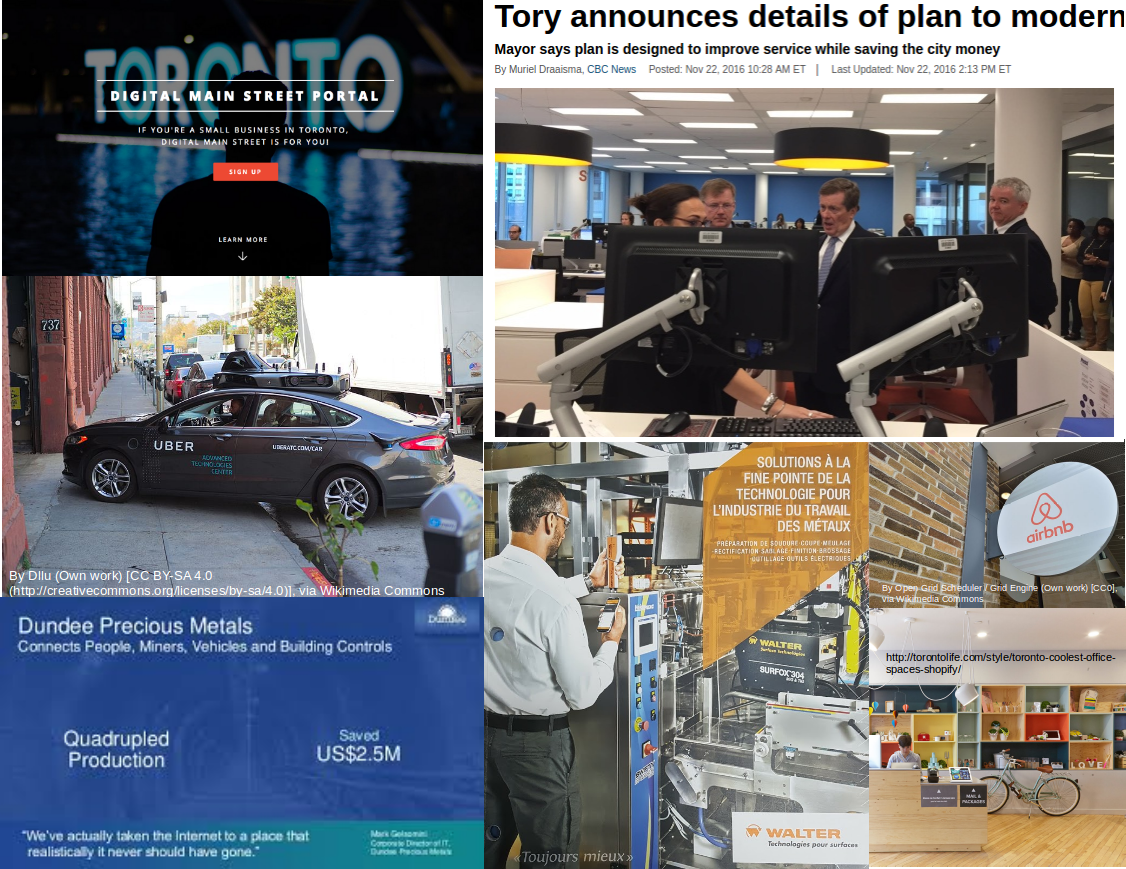
\includegraphics[width=9.5cm]{../pics/patchwork-digitization-in-Toronto}
	\end{figure}
}

\frame{
	\frametitle{Les éléments distinctifs du programme INPE}
	\begin{itemize}
		\item Formation en alternance\\ {\footnotesize($\rfrac{1}{2}$ de la semaine en salle de classe, $\rfrac{1}{2}$ chez l'employeur)}
        \pause
		\item 60--90 jours d'expérience professionnelle en position de consultant sur le numérique
        \pause
		\item Réelle valeur pour la PME: documentation des besoins, analyse, exploration et évaluation de solutions possibles
        \pause
        \item Appui des enseignants en salle de classe pour relever le défi
        \item Appui d'un réseau de mentors expérimentés (secteur bancaire, éducation, design Web, etc)
        \item Appui personnalisé du personnel local du CTIC
        \item Réalisé avec le soutien du gouvernement de l'Ontario
	\end{itemize}
}

\frame{
	\frametitle{Inauguration dans les bureaux de Microsoft}
	\framesubtitle{Présenté par Savoir-faire Linux, partenaire du CTIC}
	\begin{figure}
	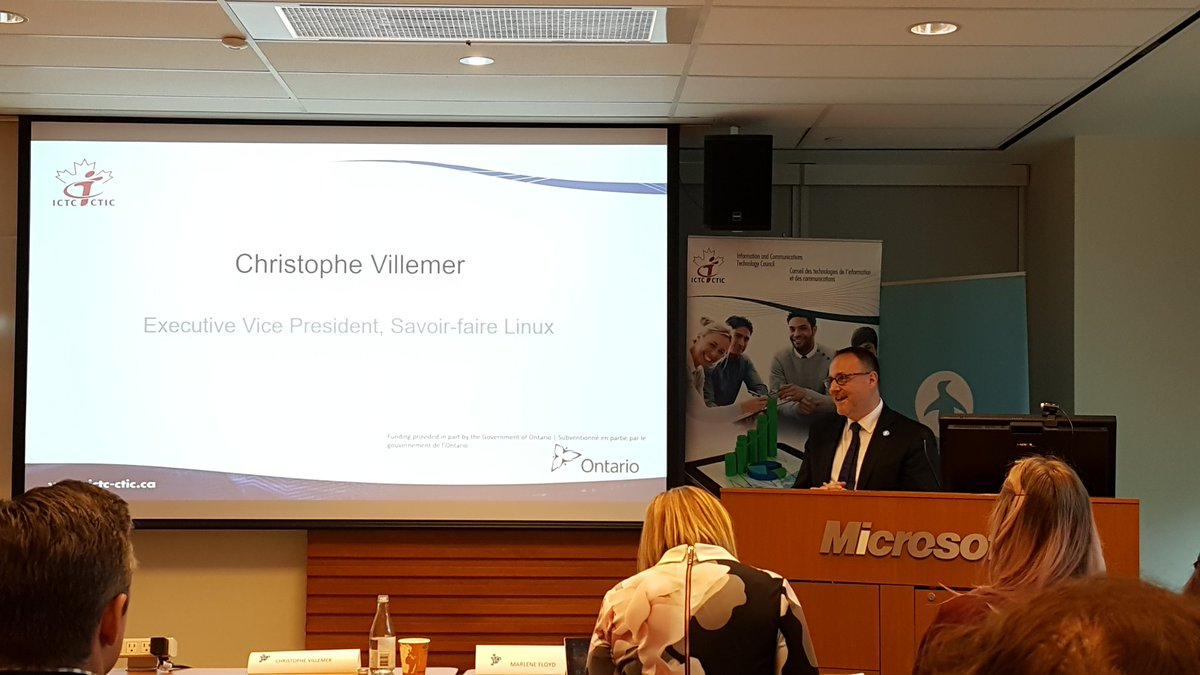
\includegraphics[height=6cm]{../pics/canadadri-20170406}
	\caption{\tiny\url{https://twitter.com/marclijour/status/849984405451964418}}
	\end{figure}
}

\frame{
	\frametitle{Inauguration en présence de l'Hon. Bardish Chagger}
	\framesubtitle{\tiny Leader du gouvernement à la Chambre des communes et ministre de la Petite Entreprise et du Tourisme}
	\begin{figure}
	
\includegraphics[height=6.5cm]{../pics/tweet-bardish_chagger_20170406}
	\caption{\tiny\url{https://twitter.com/BardishKW/status/849998821232955392}}
	\end{figure}
}

\frame{
	\frametitle{Résultats}
	\begin{itemize}
        \item Plusieurs étudiants ont été recrutés par leur employeurs
        \item Les PMEs ont lancé de nouveaux produits et services (p.~ex., commerce en ligne)
        \item Des produits primeurs ont été rendus accessibles aux territoires du nord du Canada
        \item Et une micro-brasserie a accédé à un plus grand marché... 
	\end{itemize}
}

% ======================================================================================================
%                                     Centre national d'expertise sur le Blockchain
% ======================================================================================================
\section{Autres programmes du CTIC}


\frame{
	\frametitle{Stratégie intégrée d’expérience de travail (IWES)}
	\begin{figure}
	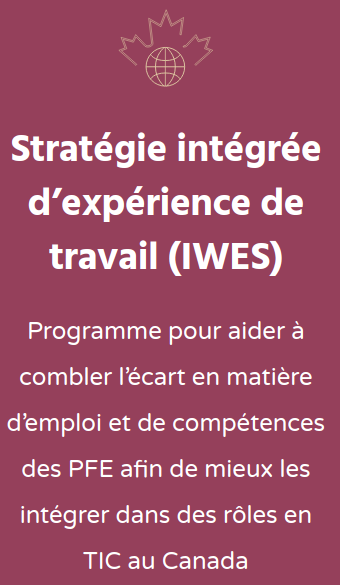
\includegraphics[height=6.5cm]{../pics/iwes}
	\caption{\tiny\url{https://www.ictc-ctic.ca/programmes-des-talents/?lang=fr}}
	\end{figure}
}

\frame{
	\frametitle{Connex’Carrière}
	\begin{figure}
	
\includegraphics[height=6.5cm]{../pics/carrierconnect}
	\caption{\tiny\url{https://www.ictc-ctic.ca/programmes-des-talents/?lang=fr}}
	\end{figure}
}

\frame{
	\frametitle{GO Talent}
	\begin{figure}
	
\includegraphics[height=6.5cm]{../pics/gotalent}
	\caption{\tiny\url{https://www.ictc-ctic.ca/programmes-des-talents/?lang=fr}}
	\end{figure}
}

\frame{
	\frametitle{Initiative d’avancement des femmes en technologie}
	\begin{figure}
	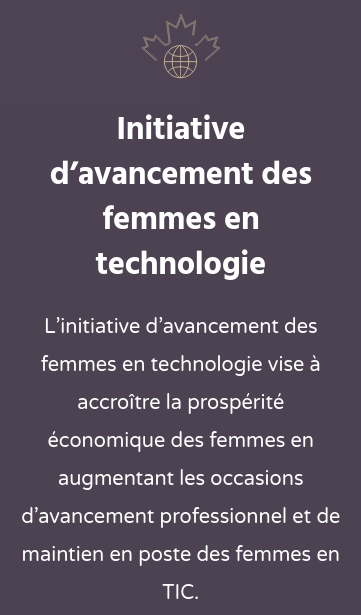
\includegraphics[height=6.5cm]{../pics/avancement-des-femmes}
	\caption{\tiny\url{https://www.ictc-ctic.ca/programmes-des-talents/?lang=fr}}
	\end{figure}
}

\frame{
	\frametitle{Le Centre national d'expertise sur le Blockchain}
	\begin{figure}
	
\includegraphics[width=11cm]{../pics/fabulousfive}
	\end{figure}
	\begin{itemize}
        \item Le CTIC, ColliderX, Blockchain Research Institute, et les deux associations canadiennes sur le blockchain
		\item Le groupe des cinq a levé 50 millions de dollars pour monter un centre national d'expertise sur le blockchain 
		\item Conversation avec la moitié des soumissionnaires sur la liste du fédéral (ISED)
		\item Initiatives visées~: programmes d'éducation, appui pour les entrepreneurs, soutien à la R\&D, etc 
	\end{itemize}
}


% ~ ~ ~ References
% ======================================================================================================
%                                     Références
% ======================================================================================================
%\section{Liens utiles}
%\frame[allowframebreaks]{
%	\frametitle{Initiative de numérisation des petites entreprises}
%	\framesubtitle{Liens utiles}
%	% keyword refers to bib file: references-KEYWORD.bib, and to the Tex file: section-KEYWORD.tex
%	\printbibliography[keyword=inpe]
%}

\end{document}

